% !TEX TS-program = pdflatex
% !TEX encoding = UTF-8 Unicode

\documentclass[a4paper, titlepage=false, parskip=full-, 10pt]{scrartcl}

\usepackage[utf8]{inputenc}
\usepackage[T1]{fontenc}
\usepackage[english, ngerman]{babel}
\usepackage{babelbib}
\usepackage{hyperref}
\usepackage{listings}
\usepackage{framed}
\usepackage{color}
\usepackage{graphicx}
\usepackage[normalem]{ulem}
\usepackage{cancel}
\usepackage{amsmath}
\usepackage{amssymb}
\usepackage{amsthm}
\usepackage{algorithm}
\usepackage{algorithmic}
\usepackage{geometry}
\usepackage{subfigure}
\geometry{a4paper, top=20mm, left=35mm, right=25mm, bottom=40mm}

\newcounter{tasknbr}
\setcounter{tasknbr}{1}
\newenvironment{task}[1]{{\bf Aufgabe \arabic {tasknbr}\stepcounter{tasknbr}} (#1):\begin{enumerate}}{\end{enumerate}}
\newcommand{\subtask}[1]{\item[#1)]}

% Listings -----------------------------------------------------------------------------
\definecolor{red}{rgb}{.8,.1,.2}
\definecolor{blue}{rgb}{.2,.3,.7}
\definecolor{lightyellow}{rgb}{1.,1.,.97}
\definecolor{gray}{rgb}{.7,.7,.7}
\definecolor{darkgreen}{rgb}{0,.5,.1}
\definecolor{darkyellow}{rgb}{1.,.7,.3}
\lstloadlanguages{C++,[Objective]C,Java}
\lstset{
escapeinside={§§}{§§},
basicstyle=\ttfamily\footnotesize\mdseries,
columns=fullflexible, % typewriter font look better with fullflex
keywordstyle=\bfseries\color{blue},
% identifierstyle=\bfseries,
commentstyle=\color{darkgreen},      
stringstyle=\color{red},
numbers=left,
numberstyle=\ttfamily\scriptsize\color{gray},
% stepnumber=5,
% numberfirstline=true,
breaklines=true,
% prebreak=\\,
showstringspaces=false,
tabsize=4,
captionpos=b,
% framexrightmargin=-.2\textwidth,
float=htb,
frame=tb,
frameshape={RYR}{y}{y}{RYR},
rulecolor=\color{black},
xleftmargin=15pt,
xrightmargin=4pt,
aboveskip=\bigskipamount,
belowskip=\bigskipamount,
backgroundcolor=\color{lightyellow},
extendedchars=true,
belowcaptionskip=15pt}

%% Enter current values here: %%
\newcommand{\lecture}{Algorithmische Geometrie SS15}
\newcommand{\tutor}{}
\newcommand{\assignmentnbr}{9}
\newcommand{\students}{Julius Auer, Alexa Schlegel}
%%-------------------------------------%%

\begin{document}  
{\small \textsl{\lecture \hfill \tutor}}
\hrule
\begin{center}
\textbf{Übungsblatt \assignmentnbr}\\
[\bigskipamount]
{\small \students}
\end{center}
\hrule

\begin{task}{Platonische Körper}
\item[]
Platonische Körper sind volkommen regelmäßige konvexe Polyeder. Polyeder sind dreidimensionale Körper, die von Polygonen (Vielecken) als Seitenflächen begrenzt sind.


\subtask{a}
Die Summe aller zusammentreffender Innenwinkel muss $< 360^\circ$ sein. Ist die Summe genau $360^\circ$ so entsteht eine Fläche in der Ebene, bei $>360^\circ$ ist die Ecke nicht mehr konvex.

Ein regelmäßiges Dreieck hat einen Innenwinkel von $60^\circ$, ein Viereck von $90^\circ$, ein Fünfeck von $108^\circ$, ein Sechseck von $120^\circ$. Ein Sechseck als Facette kann es damit nicht geben ($3\cdot120^\circ = 360^\circ$).

Somit kann es nur regelmäßige $m$-Ecke mit $m \in \{3,4,5\}$ geben.

An einer Ecke müssen $\geq 3$ Facetten zusammentreffen damit eine Ecke entsteht. So können höchstens 5 regelmäßige Dreiecke an einer Ecke zusammenstoßen ($360^\circ / 60^\circ = 6$), höchstens 3 regelmäßige Vierecke ($360^\circ / 90^\circ = 4$) und höchstens 3 regelmäßige Fünfecke ($360^\circ / 108^\circ = 3.3$). Damit ergibt sich für $k = \{3,4,5\}$, und die folgenden Kombinationen für $k$ und $m$:
$$m=3, k=3$$
$$m=3, k=4$$
$$m=3, k=5$$
$$m=4, k=3$$
$$m=5, k=3$$


\subtask{b}
Ikosaeder und Dodekaeder als geometrische Graphen 

\begin{figure}[htpb]
\begin{center}
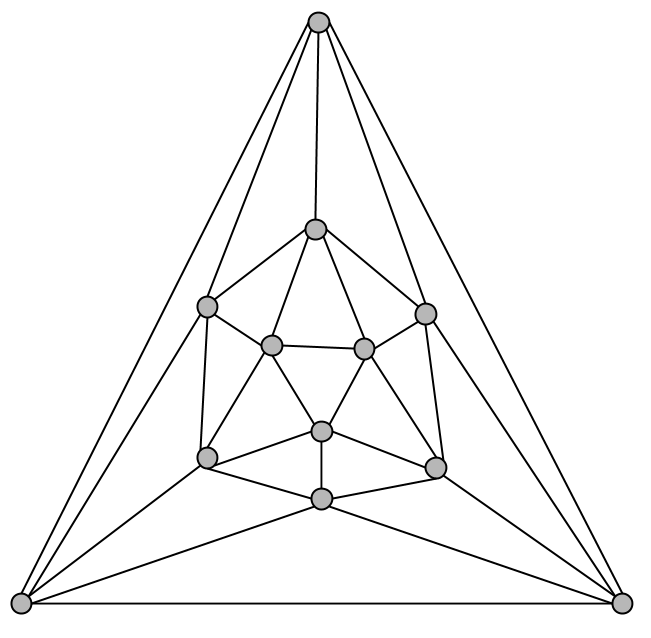
\includegraphics[width=7cm]{iko}
\end{center}
\caption{Der Ikosaeder hat 20 Facetten (gleichseitige Dreiecken), 30 Kanten und 12 Ecken.}
\end{figure}

\begin{figure}[htpb]
\begin{center}
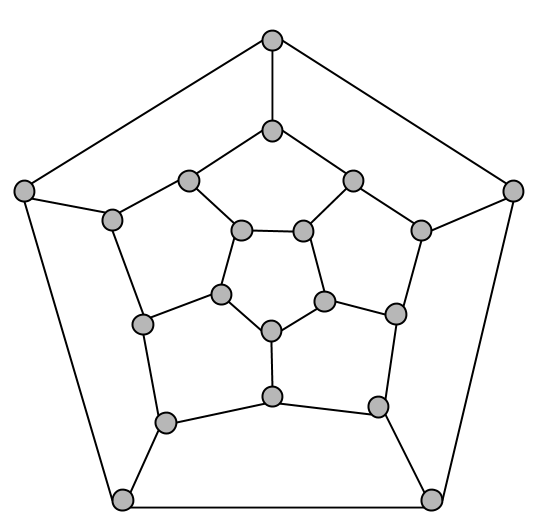
\includegraphics[width=7cm]{dode}
\end{center}
\caption{Der Dodekaeder hat 12 Facetten (regelmäßiges Fünfeck), 30 Kanten und 20 Ecken.}
\end{figure}




\end{task}

\begin{task}{d-dimensionale Polytope}
\subtask{a}
Seien $V_d$ die Ecken des Einheitswürfels in $d$ Dimensionen. Dann gibt es für jede Ecke $(x_1,...,x_d)$ dieses Würfels in $d+1$ Dimensionen genau die zwei Ecken $(x_1,...,x_d,0)$ und $(x_1,...,x_d,1)$. Es gilt also:
$$|V_{d+1}|=2\cdot |V_d|$$
Dass $|V_1|=2$ ist klar, womit sich die Anzahl Ecken im Allgemeinen ergibt, zu:
$$|V_d|=2^d$$ 

Für den Einheitswürfel liegt eine Facette $f$ stets parallel zu einer Achse des Koordinatensystems. Für jede Dimension gibt es zwei solcher paraller Facetten und folglich ist für die Menge aller Facetten $F_d$ somit
$$|F_d|=2\cdot d$$
Die jeweiligen Facetten $f_1,...,f_{2\cdot d}\in F_d$ seien dabei durch die sie begrenzenden Ecken definiert:
$$f_i=\begin{cases}
\{ (x_1,...,x_{i\text{ mod } d},...,x_d)\in V_d:x_i=0\}&\text{, falls }i\le d\\
\{ (x_1,...,x_{i\text{ mod }d},...,x_d)\in V_d:x_i=1\}&\text{, sonst}
\end{cases}$$

\subtask{b}
Siehe Abb. \ref{fig:2.b}: Ecken mit $x_4=1$ sind mit dem Faktor $\frac{1}{3}$ skaliert, um $(0.4,0.3,0,0)$ verschoben und haben eine andere Farbe. Kanten, deren Eckpunkte unterschiedliche Werte in dieser Dimension haben, sind Wellenförmig dargestellt (durch eine gerade Kante zu implizieren es gäbe einen anschaulichen geometrischen Zusammenhang in einer derartigen dreidimensionalen Darstellung des $W_4$, wäre doch Humbug !?)

\begin{figure}[h!]
\begin{center}
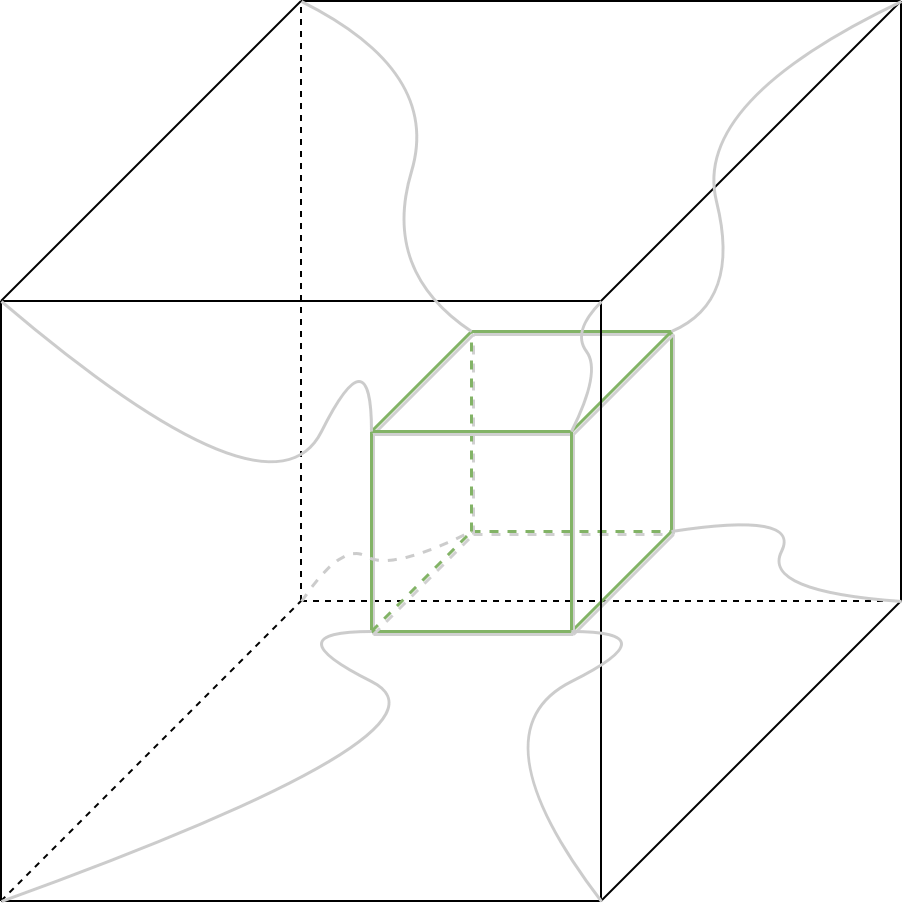
\includegraphics[width=8cm]{cube4d}
\end{center}
\caption{$W_4$}
\label{fig:2.b}
\end{figure}

\subtask{c}
Alle Punkte mit einer Koordinate $<0$ liegen außerhalb des Simplex. Im positiven Sektor wird das Simplex begrenzt durch eine Hyperebene. Der Bereich der von den Koordinatenachsen und dieser Hyperebene eingeschlossen wird ist genau das Simplex. Die Ecken des Simplex sind somit stets $0^d$ und die $d$ vielen Ecken die benötigt werden, um die Hyperebene zu definieren (das sind genau die Ecken $(1,0,...,0),...,(0,...0,1)$). Es gibt also $d+1$ viele Ecken.

Offenbar entstehen so stets $d+1$ viele Facetten (der ''Boden'' und $d$ viele, die inzident zu $0^d$ sind). Die Ecken, welche die Hyperebene beschreiben, sind zwar paarweise adjazent, liegen jedoch alle auf besagter Hyperebene, weshalb keine zusätzlichen Facetten entstehen. Für $S_4$ (siehe auch Abb. \ref{fig:2.c}) liegt beispielsweise $p_4$ auf der selben Facette wie $p_1,...,p_3$.

\begin{figure}[h!]
\begin{center}
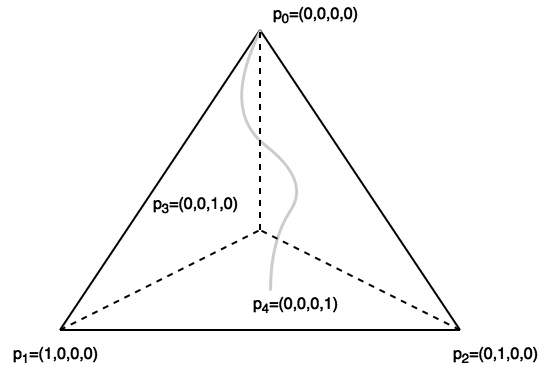
\includegraphics[width=8cm]{simplex4d}
\end{center}
\caption{$S_4$ - man sieht deutlich 5 Facetten :)}
\label{fig:2.c}
\end{figure}
\end{task}

\begin{task}{Konvexe Hülle}
\item[]
Wir gehen davon aus, dass keine 4 Punkte auf einer Ebene liegen. Die Punkte $p_1, \dots, p_n$ werden nacheinader hinzugefügt. In jedem Schritt wird die konvexe Hülle aktualisiert. Wir nehmen nun an, dass die konvexte Hülle der ersten $k$ Punkte bekannt ist. $p_{k+1}$ kann nun entweder (1) Teil der konvexen Hülle sein, $p_{k+1} \in CH(p_1, \dots, p_n)$ oder (2) außerhalb der konvexen Hülle liegen, $p_{k+1} \not \in CH(p_1, \dots, p_n)$.

\newpage
Für jeden Punkt $p_i$ der bereits zur konvexen Hülle gehört wird nun getestet, mit welchen Facetten die Gerade $g$ durch $p_i$ und $p_{k+1}$ einen Schittpunkt hat. Treten keine Schnittpunkte auf so ist die Strecke $p_i, p_{k+1}$ eine neue Kante. Der Punkt $p_i$ wird für das spätere Erzeugen der Facetten geeignet abgespeichert, nennen wir die Menge $F$. Alle Facetten die von $g$ \emph{getroffen} wurden, können entfernt werden.

Aus je zwei benachbarten Knoten in $P_n$ und $p_{k+1}$ wird nun eine neue Facette gebastelt.

\begin{algorithm}
\caption{$CH3D(P = \{p_1, p_2, \dots, p_n\})$}
\begin{algorithmic}[1]
\STATE $C \leftarrow CH(p_1, p_2, p_3, p_4)$
\FOR {$i=5$ \TO $n$}
    \IF{$p_i$ liegt außerhalb von $C$}
    		\FOR { alle Punkte $p_c \in C$}
        		\FOR { alle Facetten $f_c \in C$ }
		        		\IF {Gerade durch $p_i$ und $p_c$ schneidet Facette $f_c$}
		        				\STATE entferne $f_c$ aus $C$ (und zugehörige Kanten und Ecken bzw. Punkte)\\
		        		\ELSE
		        				\STATE füge $p_i, p_c$ als neue Kante zu $C$ hinzu\\
		        				\STATE $F \leftarrow p_c$ (merken)\\
		        		\ENDIF
        		\ENDFOR
    		\ENDFOR
    \ENDIF
    \STATE füge $p_i$ als neue Ecke bzw. Punkt zu $C$ hinzu\\
		\FOR {alle benachbarten Knoten $\in F$ }
				\STATE erzeuge neue Facette 
		\ENDFOR
\ENDFOR 
\end{algorithmic}
\end{algorithm}

(2) Anzahl der Punkte: $O(n)$\\
(3) Test ob inner oder außerhalb???\\
(4) Anzahl Punkte in konvexer Hülle: $O(n^2)$\\
(5) Anzahl der Facetten $O(n)$\\
(6-10) $O(1)$\\
(6-10) $O(1)$\\
(15) $O(1)$\\
(16, 17) $O(n)???$

Gesamtlaufzeit in $O(n \cdot (n^2 \cdot n + n)) = O(n^4)$.

Zweiter Versuch - naiv, einfach zu beschreiben, Brute-Force:

(1) Für jedes Tupel $(p_1,p_2,p_3)$ paarweise ungleicher $p_1,p_2,p_3\in S$:\\
(2) Prüfe ob alle Punkte $p\in S$ auf der selben Seite der Ebene liegen, die von  $(p_1,p_2,p_3)$ aufgespannt wird. Wenn dem so ist gehören $(p_1,p_2,p_3)$ zur konvexen Hülle (wenn keine 4 Punkte auf einer Ebene liegen definieren sie außerdem eine Facette).

Es gibt $|S|^3$ Tupel die in (1) betrachtet werden müssen. Für (2) müssen wiederum alle $|S|$ Elemente geprüft werden. Insgesamt ist folglich $O(|S|^4)$ Zeit erforderlich.
\end{task}
\end{document}